%
% beispiele.tex %% Beispiele partieller Differentialgleichungen
%
% (c) 2008 Prof Dr Andreas Mueller
%
\chapter{Einführende Beispiele partieller Differentialgleichung\label{chapter-beispiele}}
\lhead{Einführende Beispiele}
In diesem Kapitel sollen einige Beispiele von Differentialgleichungen
dargestellt werden, die später zur Illustration der allgemeinen
Gesetze und der Lösungstechniken verwendet werden können.
Die Beispiele illustrieren
\begin{enumerate}
\item die vielfältigen Anwendungen der Theorie der partiellen 
Differentialgleichungen,
\item drei grundsätzlich verschiedene
Situationen, die jedoch alle in den Anwendungen auftreten, und
\item die Bedeutung und die möglichen Formen von Anfangs-
und Randbedingungen.
\end{enumerate}

\rhead{Wellengleichung}
\section{Wellengleichung\label{beispiele:wellengleichung}}
\index{Wellengleichung}
In der einfachsten Form beschreibt diese Gleichung die Schwingungen der
Saite einer Gitarre oder eines Klaviers, oder der Luftsäule eines
Blasinstrumentes.
\index{Klavier}
\index{Gitarre}
\index{Luftsaule@Lufts\äule}
\index{Blasinstrument}
Natürlich ist sie auch anwendbar auf einen schwingenden
Balken, oder, in auf mehrere Dimensionen verallgemeinerter Form auf
schwingende Platten, die Schallausbreitung in einem Raum oder die Schwingungen
einer beliebigen dreidimensionalen Struktur.
\index{Balken}
\index{Platte}
Und selbstverständlich
lassen sich damit auch andere Wellen\-phä\-no\-mene modellieren:
elektromagnetische Wellen (Licht, Radio) oder flache Wellen an der
Wasseroberfläche.
\index{Welle!elektromagnetisch}
\index{Wasserwellen}

\subsection{Die Differentialgleichung der schwingenden Saite\label{beispiele:schingende-saite}}
\index{Saite}
Eine dünne Saite mit der linearen Massedichte $\mu$ sei zwischen den
Punkten $x=0$ und $x=l$ eingespannt. An den Enden der Saite wirkt eine
Kraft $F$. Wir suchen die Differentialgleichung, die die Bewegung der Saite
beschreibt, nachdem wir die Saite in eine bestimmte Form gebracht, und
zur Zeit $t=0$ losgelassen haben.

Offenbar können wir den momentanen Zustand der Saite mit Hilfe einer
Funktion $u(x,t)$ beschreiben, welche die Auslenkung der Saite
am Punkt $x$ zur Zeit $t$ angibt. Die Lösung des Problems besteht darin,
eine Differentialgleichung für die Funktion $u$ zu finden.

Aus dieser Beschreibung des Problems können wir die Anfangsbedingungen zur
Zeit $t=0$ und die Randbedingungen für alle Zeiten $t\ge 0$ bereits ableiten.
Zur Zeit $t=0$ ist die Form der Saite vorgegeben. Es gibt also eine Funktion
$f(x)$, welche nicht von der Zeit abhängt, und die mindestens stetig
sein muss (weil die Saite sonst reisst). Die gesuchte Lösung $u$
muss erfüllen:
\[
u(x,0)=f(x).
\]
Da die Saite sich an ihren Enden nicht bewegen kann, muss die Funktion
$u$ dort für alle Zeiten den Wert $0$ haben:
\[
u(0,t)=u(l,t)=0\quad\forall t\ge 0.
\]

\begin{figure}
\begin{center}
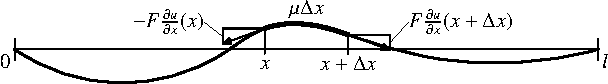
\includegraphics[width=\hsize]{../common/images/saite-1}
\end{center}
\caption{Ableitung der Differentialgleichung der schwingenden Saite\label{saite}}
\end{figure}
Für die Ableitung der Bewegungsgleichung der Saite betrachten wir den
Ausschnitt zwischen $x$ und $x+\Delta x$ der Saite (Abbildung \ref{saite}).
Er hat die Masse
$\mu \Delta x$. Für die Beschleunigung dieses Abschnittes sind die
Kräfte zuständig, die senkrecht auf der $x$-Achse stehen. Die Kraft längs
der Seite ist nach Voraussetzung $F$, die Steigung gibt an, welcher Teil
dieser Kraft senkrecht auf die $x$-Achse wirkt. Insgesamt wirkt auf den
Abschnitt zwischen $x$ und $x+\Delta x$ die Kraft
\[
F\frac{\partial u}{\partial x}(x+\Delta x)-F\frac{\partial u}{\partial x}(x).
\]
Mit der Beschleunigung $\frac{\partial^2u}{\partial t^2}$ wird die
Bewegungsgleichung
\begin{align*}
\mu\Delta x\frac{\partial^2u}{\partial t^2}(x)&=
F\frac{\partial u}{\partial x}(x+\Delta x)-F\frac{\partial u}{\partial x}(x)\\
\Rightarrow\qquad
\frac{\mu}{F}\frac{\partial^2u}{\partial t^2}(x)&=
\frac1{\Delta x}\left(\frac{\partial u}{\partial x}(x+\Delta x)-\frac{\partial u}{\partial x}(x)\right)
\end{align*}
Geht man zum Grenzwert $\Delta x\to 0$ über, findet man die
partielle Differentialgleichung
\[
\frac{\partial^2u}{\partial t^2}=\frac{F}{\mu}\frac{\partial^2u}{\partial x^2}.
\]
Der Koeffizient $\frac{F}{\mu}$ hat die Dimension einer Geschwindigkeit im
Quadrat, es handelt sich um die Ausbreitungsgeschwindigkeit der Wellen entlang
der Saite.

\subsection{Die Differentialgleichung einer Orgelpfeife\label{beispiele:orgelpfeife}}
\index{Orgelpfeife}
\index{Luftdruck}
Grundsätzlich ist die Analyse der schwingenden Saite auch auf
eine Orgelpfeife anwendbar. Die Rolle der Auslenkung übernimmt
hier der Luftdruck $p(x,t)$. Eine ähnliche Argumentation wie bei
der schwingenden Saite führt uns erneut auf die Wellengleichung:
\[
\frac{\partial^2p}{\partial t^2}=
a^2\frac{\partial^2p}{\partial x^2}
\]
Darin ist $a$ die Ausbreitungsgeschwindigkeit.

Die Randbedingungen sind jedoch etwas vielseitiger.
Ist die Pfeife am Ende geschlossen, man spricht von
einer gedackten Pfeife, kann sich die Luft an diesem Ende nicht bewegen.
Damit sich die Luft in Bewegung versetzt, muss ein Druckunterschied herschen,
die Beschleunigung der Luft ist proportional zum Druckgradienten
$\frac{\partial p}{\partial x}$. Umgekehrt muss als an Stellen, wo die
Luft sich gar nicht bewegen kann, der Druckgradient verschwinden.
Die Randbedingung am geschlossenen Ende ist daher
\[
\frac{\partial p}{\partial x}=0.
\]

Bei einer offenen Pfeife hingegen kann sich die Luft am Ende beliebig
bewegen, der Gradient kann daher jeden beliebigen Wert annehmen.
Anderseits kann man auch nicht fordern, dass der Druck am
Ende der Pfeife genau den Umgebungsdruck hat, da ja hörbar eine
Schallwelle abgestrahlt wird, die genau diese Druckschwankungen am
Ende der Pfeife weitertransportiert. Allerdings sind diese Druckschwankungen
wesentlich geringer als die Druckschwankungen im inneren des Rohres.

Insgesamt erkennen wir, dass mögliche Randbedingungen für dieses Problem
beliebig aus einer Bedingung an den Wert am Rand und einer Bedingung
an die Ableitung am Rand kombiniert werden kann.

\subsection{Wellengleichung in zwei und drei Dimensionen\label{beispiele:wellengleichung2d}}
Analog zur Differentialgleichung einer schwingenden Saite kann
man auch die Differentialgleichung einer am Rand eingespannten Membran
ableiten.
\index{Membran}
Sei $G$ ein Gebiet in $\mathbb R^2$, und sei $\gamma$ der Rand
von $G$, $\gamma = \partial G$. Die Schwingungen einer entlang der Randkurve
$\gamma$ eingespannte Membran wird beschrieben durch eine Funktion
\[
 u \colon G\times \mathbb R_{t \ge 0}\to\mathbb R\colon (x,y,t)\mapsto  u (x,y,t)
\]
die die Auslenkung der Membran aus der Ruhelange angibt. Das Problem ist aber
erst bestimmt, wenn wir die Auslenkung der Membran zur Zeit $t=0$ kennen,
diese kann durch eine im Gebiet $G$ definierte Funktion $f(x,y)$ beschrieben
werden.

Die Funktion $ u $
erfüllt die Differentialgleichung
\[
\frac{\partial^2 u }{\partial t^2}
=c^2\left(\frac{\partial^2 u }{\partial x^2}+\frac{\partial^2 u }{\partial y^2}\right),
\]
die Randbedingung
\[
 u (x,y,t)=0\qquad \forall (x,y)\in\gamma,t\ge 0,
\]
und die Anfangsbedingung
\[
 u (x,y,0)=f(x,y)\qquad \forall (x,y)\in G.
\]
Die Konstante $c$ ist die Ausbreitungsgeschwindigkeit der Wellen in der Membran.

In drei Dimensionen lautet
die Wellengleichung 
\[
\frac{\partial^2 u }{\partial t^2}
=c^2\left(\frac{\partial^2 u }{\partial x^2}
+\frac{\partial^2 u }{\partial y^2}
+\frac{\partial^2 u }{\partial z^2}
\right).
\]
Auch für dieses Problem sind weitere Angaben notwendig, damit das Problem
wohl gestellt ist.
Zunächst ist ein Gebiet $G\subset \mathbb R^3$ festzulegen, welches
eine geeignet glatte Randfläche hat.
Die Lösung $ u (x,y,z,t)$ ist definiert für Punkte $(x,y,z)\in G$
und für Zeitpunkte $t\ge 0$.
Der Anfangszustand ist eine Funktion $f(x,y,z)$,
definiert auf $G$.

\subsection{Der Laplace-Operator\label{beispiele:laplaceoperator}}
In allen bisher diskutierten Problemen tritt der Laplace-Operator
\[
\Delta
=
\begin{cases}
\displaystyle
\frac{\partial^2}{\partial x^2}
+\frac{\partial^2}{\partial y^2}&\qquad\text{2 Dimensionen}\\
\\
\displaystyle
\frac{\partial^2}{\partial x^2}
+\frac{\partial^2}{\partial y^2}
+\frac{\partial^2}{\partial z^2}&\qquad\text{3 Dimensionen}
\end{cases}
\]
auf. Tatsächlich ist er bis auf einen konstanten Faktor der einzige Ausdruck
in den zweiten partiellen Ableitungen, der bei beliebigen Drehungen des
Koordinatensystems erhalten bleibt.
Auch zeigt sich in der Differentialgeometrie, dass der Laplace-Operator
eng mit der Geometrie des Raumes verknüpft ist.

\section{Poisson-Problem}
\rhead{Poisson-Problem}

\subsection{Minimalflächen\label{beispiele:minimalflaechen}}
Welche Form nimmt eine Seifenhaut ein, die am Rande $\gamma$ eines
zweidimensionalen Gebietes $G$ auf die Höhe $f(x,y)$ mit $(x,y)\in \gamma$
angehoben wird? Wir beschreiben die Seifenhaut durch eine Funktion
$ u (x,y)$, natürlich muss gelten $ u (x,y)=f(x,y)$ für alle
Punkte $(x,y)\in\gamma$.
Im Gleichgewicht wird die Membran so geformt, dass die Kräfte
der Oberflächenspannung sich an jeder Stelle der Seifenhaut gegenseitig
aufheben. Betrachtet man nur die $x$-Richtung, ist die Kraft auf die
Seifenhaut durch die zweite Ableitung in $x$-Richtung geben.
Diese Kraft muss durch Kraft kompensiert werden, die durch die
zweite Ableitung von $ u $ in $y$-Richtung hervorgerufen wird.
Die Funktion $ u $ muss also die Gleichung
\[
\frac{\partial^2 u }{\partial x^2}+\frac{\partial^2 u }{\partial y^2}
=\Delta u =0.
\]
Dieses einfache Argument ist auf den ersten Blick einleuchtend, bräuchte
aber eine noch etwas genauere Rechtfertigung. Darauf wollen wir allerdings
verzichten.

\subsection{Elektrisches Potential\label{beispiele:elektrischespotential}}
In der Elektrizitätslehre wird gezeigt, dass das elektrostatische Feld 
ein Gradientenfeld ist. Der Gradient des Potentials $\varphi$  ist das
elektrische Feld:
\[
\vec E=\operatorname{grad}\varphi.
\]
Andererseits wird auch gezeigt, dass die Quellen des elektrische Feldes die
Ladungen sind, dass also insbesondere das elektrische Feld im Vakuum quellenfrei ist.
Die Divergenz von $\vec E$ muss also verschwinden, oder
\[
\operatorname{div}\vec E=\operatorname{div}\operatorname{grad}\varphi
=\Delta \varphi=0.
\]
Dies zeigt, dass wenigstens mathematisch ein enger Zusammenhang zwischen
einer gespannten Gummihaut und einem elektrischen Potential herrscht.
Als Modell für ein Potential ist die Gummihaut daher eine bessere
Näherung, als auf den ersten Blick scheinen mag.

\rhead{Wärmeleitungsgleichung}
\section{Wärmeleitungsgleichung\label{beispiele:waermeleitung}}
\index{Warmeleitungsgleichung@W\ärmeleitungsgleichung}
Die Wärmeleitungsgleichung ist der Prototyp einer parabolischen partiellen
\index{Differentialgleichung!partielle!parabolische}
Differentialgleichung. Sie kann auch verwendet werden, um Diffusionsprozesse
zu beschreiben. Lässt man komplexe Werte der Konstanten zu, entpuppt
sie sich sogar als die Grundgleichung der Quantenmechanik.

Wir leiten die Wärmeleitungsgleichung im eindimensionalen Fall ab, und stellen
uns dazu einen wärmleitenden dünnen Stab der Länge $l$ vor. Punkte
entlang des Stabes haben die Koordinaten $x$ zwischen $0$ und $l$.
Die Temperaturverteilung in diesem Stab zur Zeit $t=0$ ist eine Funktion
$f(x)$. Wir suchen die Temperaturverteilung zu einem beliebigen späteren Zeitpunkt.

Wir suchen also eine Funktion $T(x,t)$ und erwarten natürlich, dass sie
genügend glatt ist, dass wird das Problem mit Hilfe einer partiellen
Differentialgleichung behandeln können. Die pro Zeiteinheit
durch die Querschnittsfläche an der Stelle $x$ fliessende Wärmemenge ist
proportional zur Ableitung $\frac{\partial T}{\partial x}$.
Die Wärmemenge im Teilstück zwischen $x$ und $x+\Delta x$ ändert sich also
pro Zeitenheit um einen Betrag, der proportional ist zu
\[
\frac{\partial T}{\partial x}(x+\Delta x)-\frac{\partial T}{\partial x}(x).
\]
Im Grenzwert $\Delta x\to 0$
ändert sich die Energiedichte also pro Zeiteinheit um einen zu
\[
\lim_{\Delta x\to 0}\frac1{\Delta x}\left(\frac{\partial T}{\partial x}(x+\Delta x)-\frac{\partial T}{\partial x}(x)\right)
=\frac{\partial^2T}{\partial x^2}
\]
proportionalen Betrag.
Die Temperatur ist aber propertional zur Energiedichte, also ist die Änderung
der Energiedichte auch proportional zur Änderung der Temperatur:
\[
\frac{\partial T}{\partial t}=a^2\frac{\partial^2T}{\partial x^2}.
\]
In der Physik lernt man, dass
\[
a=\sqrt{\frac{k}{c\varrho}},
\]
darin ist $k$ das Wärmeleitvermögen, $c$ die spezifische Wärme
und $\varrho$ die Dichte.

Auch für dieses Problem müssen Anfangs und Randbedingungen formuliert werden.
Als Anfangsbedinung wurde bereits die Funktion $f(x)$ vorgegeben, es muss
gelten
\[
T(x,0)=f(x)\qquad \forall x\in[0,l].
\]
Als Randbedingen kommen wiederum Bedingungen an die Temperatur oder an die
Ableitung am Rande in Frage.

Vorgabe der Temperatur an den Stellen $x=0$ und $x=l$ bedeutet physikalisch, dass
die Enden von einem externen Wärmebad auf konstanter Temperatur gehalten
werden. Die Steigung von $T$ kann an dieser Stelle beliebige Werte annehmen,
sie gibt an, wie viel Wärme durch die Enden fliesst.

Vorgabe der Steigung an den Stellen $x=0$ und $x=l$ bedeutet physikalisch,
dass man den Wärmefluss in oder aus dem Stab an dessen Enden vorgibt.

\rhead{Überschallströmung}
\section{Überschallströmung \label{beispiele:ueberschall}}
Im Jahre 1928 habilitierte sich Jakob Ackeret an der ETH mit einer
Schrift mit dem Titel ``Über Luft-Kräfte bei sehr grossen
Geschwindigkeiten insbesondere bei ebenen Strömungen''. Darin
zeigt er, wie mit einer linearen Näherung die Luftkräfte
in einer Überschallströmung berechnet werden können.
Die Geschwindigkeit des mit Geschwindigkeit $v_1$ in $x$-Richtung
anströmenden
Gases wird dabei als Gradient einer Funktion $\varphi$ gesucht,
es stellt sich heraus, dass die Funktion $\varphi$ die Gleichung
\[
(1-Ma_1)\frac{\partial^2\varphi}{\partial x^2}
+
\frac{\partial^2\varphi}{\partial y^2}
+
\frac{\partial^2\varphi}{\partial z^2}=0
\]
erfüllt.
Darin ist $Ma_1=\frac{v_1}{c_1}$, $c_1$ ist die Schallgeschwindigkeit.

Für kleine Geschwindigkeiten ist $(1-Ma_1)>0$, die Gleichung ähnelt
der Poissongleichung, man spricht in diesem Fall von einer
``Potentialströmung''.
Für Überschallgeschwindigket ist jedoch $(1-Ma_1) < 0$,
diese Differentialgleichung ähnelt eher der Wellengleichung.
Wir können daraus bereits schliessen, dass mindestens in linearer
Näherung das Strömungsbild und auch die Luftwiderstandsverhältnisse
sich grundlegend unterscheiden müssen.
Tatsächlich wird das Strömungsbild im Überschallbereich dominiert
von den Schockwellen (Wellengleichung!), welche die Energie mit
Schallgeschwindigkeit vom umströmten Körper wegtransportieren
(Abbildung~\ref{ueberschall2d}).

\rhead{Balkengleichung}
\section{Balkengleichung\label{beispiele:balkengleichung}}
\index{Balken}
\index{Balkengleichung}
\index{Biegung}
Bei der Herleitung der Differentialgleichung einer Saite haben
wir verwendet, dass sich die Saite der Biegung nicht wiedersetzt.
Selbst eine beliebig starke Biegung hat keine Kraft zur Folge, die
die Biegung wieder strecken würde.
Ein Balken verhält sich jedoch ganz anders. Bei der Biegung entstehen
innere Spannungen im Material, welche den Balken wieder in die
gerade Ausgangslage zu bringen versuchen.
Wie diese Kräfte entstehen, ist nicht Gegenstand dieser Vorlesung.
Es ist aber klar, dass die Spannungen umso grösser sein werden,
je grösser die Krümmung des Stabes ist. Sie sind auch proportional
zu einer Materialkonstanten, dem Elastizitätsmodul $E$ und der
\index{Elastizitatsmodul@Elastizit\ätsmodul}
Gestalt des Querschnittes, ausgedrückt durch das Flächenträgheitsmoment
\index{Flachentragheitsmoment@Fl\ächentr\ägheitsmoment}
$I$\footnote{Falls Ihnen das Flächenträgheitsmoment nicht bekannt ist,
spielt das für die weitere Diskussion keine Rolle.}.

Um die Gleichung eines schwingenden Stabes aufzustellen, brauchen wir
die Kräfte, die den Balken in die Ruhelage zu bringen versuchen. Sei
$w(x,t)$ die Auslenkung des Balkens aus der Ruhelage zur Zeit $t$
und an der Stellen $x$. Der Balken soll die lineare Dichte $m$ haben.
Ein Element der Länge $\Delta x$ des Balkens erfährt dann die
folgenden Kräfte:
\begin{enumerate}
\item Rücktreibende Kräfte durch die Spannung des Balkens: $-EI\frac{\partial^4}{\partial^4 x}w(t,x)\Delta x$
\item Dämpfung $-b\frac{\partial}{\partial t}w(t,x)\Delta x$
\item Äusser Kräfte (zum Beispiel Belastungen des Balkens) $q(x,t)\Delta x$
\end{enumerate}
Nach dem Newtonschen Gesetz müssen sich diese Kräfte zu
\[
m\Delta x\frac{\partial^2}{\partial^2 t}w(t,x)
\]
summieren. Es gilt also pro Element des Balkens
\begin{align*}
m\frac{\partial^2}{\partial^2t}w(t,x)
&=-EI\frac{\partial^4}{\partial^4x}w(t,x)-b\frac{\partial}{\partial t}w(t,x)+q(t,x)
\\
EI\frac{\partial^4}{\partial^4x}w(t,x)
+b\frac{\partial}{\partial t}w(t,x)
+m\frac{\partial^2}{\partial^2t}w(t,x)
&=q(t,x)
\end{align*}
Für die Bewegung eines Balkens gilt also eine partielle Differentialgleichung.

\rhead{Plattengleichung}
\section{Plattengleichung\label{beispiele:plattengleichung}}
\index{Plattengleichung}
Noch etwas komplizierter ist die Berechnung einer Platte. Im Gegensatz
zu einer Membran versuchen die Spannungen, die bei der Verbiegung der
Platte unter Last entstehen, die Platte wieder in die Ausgangslage zurück
zu bringen. Die Gleichung einer an der Stelle $(x,y)$ um den Betrag
$w(x,y)$ aus der $x$-$y$-Ebene ausgelenkten Platte ist
\[
D\left(
\frac{\partial^2}{\partial^2 x}
+
\frac{\partial^2}{\partial^2 y}
\right)
\left(
\frac{\partial^2}{\partial^2 x}
+
\frac{\partial^2}{\partial^2 y}
\right)
w(x,y)
=D\Delta\Delta w(x,y)
=p(x,y),
\]
wobei $D$ eine Materialkonstante ist und $p(x,y)$ der Druck, der
an der Stelle $(x,y)$ auf die Platte drückt.

\section{Zusammenfassung: Das Wichtigste in Kürze\label{beispiele:zusammenfassung}}
\begin{enumerate}
\item In der Physik treten partielle Differentialgleichungen meistens
bei der Beschreibung von Feldern auf: Wellen (\ref{beispiele:wellengleichung},
Druck (\ref{beispiele:orgelpfeife}),
Temperatur (\ref{beispiele:waermeleitung}),
Geschwindigkeit (\ref{beispiele:ueberschall}), Potential,
elektrisches Feld (\ref{beispiele:elektrischespotential}), \dots
\item Sehr häufig tritt dabei der Laplace-Operator auf (\ref{beispiele:laplaceoperator}).
\end{enumerate}
